% Preamble
\documentclass[12pt,a4paper]{article}
\usepackage{enumerate} 	
\usepackage{setspace}						
\usepackage{authblk}	
\usepackage{graphicx} 	
%\usepackage[nomarkers, nolists]{endfloat} 
\usepackage{pdflscape}	
\usepackage{mathtools}	
\usepackage[osf]{mathpazo} 
\usepackage{lineno} 	
\usepackage{hyperref}
\usepackage[round]{natbib} 
\usepackage{setspace}
\usepackage{longtable}
\usepackage{fancyhdr}

\setcounter{secnumdepth}{0} 
%\raggedright 			
%\pagenumbering{arabic}	
\pagenumbering{gobble}

\pagestyle{fancy}
\rhead{\textit{Guillerme \& Cooper 2018}}
\lhead{\textit{Supporting Information: S1}}
\renewcommand{\headrulewidth}{0pt}
\renewcommand{\footrulewidth}{0pt}
\setlength{\headsep}{0.3in}

\renewcommand{\thetable}{A\arabic{table}}
\renewcommand{\thefigure}{A\arabic{figure}}

% First order headings upper case bold
\usepackage{titlesec}
\titleformat*{\section}{\small\bfseries\uppercase}

% Second order headings normal case italics
\titleformat*{\subsection}{\small\itshape}

% Third order, italics, paragraph style
\titleformat*{\paragraph}{\small\itshape}

\begin{document}

\par{\centering{\Large \bf Supporting Information from ``Time for a rethink: time sub-sampling methods in disparity-through-time analyses''\par}}

\setlength{\parindent}{1cm}

\section{Appendix S1: Additional details of datasets}

\subsection{Beck2014 (Figure \ref{figure:beck})}
The following taxa were removed because they were in the phylogeny but not the character matrix or vice versa: \textit{Montanalestes}, \textit{Lainodon}, \textit{Kharmerungulatum}, \textit{Alymlestes}. 

\subsection{Brusatte2014 (Figure \ref{figure:brusatte})} 
We used one randomly selected time-scaled tree from Brusatte et al. (2014).
Zero-length branches were replaced with the minimum branch length in the phylogeny.
The following taxa were removed because they were in the phylogeny but not the character matrix or vice versa: \textit{Sinraptor dongi}, \textit{Hesperonychus elizabethae}, \textit{Pyroraptor olympius}, \textit{Limenavis patagonica}, \textit{Lithornis}, \textit{Crypturellus undulatus}, \textit{Gallus gallus}, \textit{Crax pauxi}, \textit{Anas}\\ \textit{platyrhynchus}, \textit{Chauna torquata}, \textit{Epidendrosaurus} and \textit{Kinnareemimus}. 
The following taxa were removed because they shared no characters in the morphological matrix: \textit{Shanag ashile}, \textit{Atrociraptor marshalli}, \textit{Proceratosaurus bradleyi}, \textit{Incisivosaurus gauthieri}, \textit{Enigmosaurus}, \textit{Nanshiungosaurus brevispinus}, \textit{Xixiasaurus}, \textit{Tsaagan mangas}, \textit{Mirischia}, \textit{Pedopenna}, \textit{Suzhousaurus}, \textit{Juratyrant}, \textit{Vorona}, \textit{Bonapartenykus}, \textit{Teratophoneus}, \textit{Gobipteryx}, \textit{Songlingornis}, \textit{Liaoningornis longidigitu} and \textit{Achillesaurus}.   

\subsection{Bapst2016 (Figure \ref{figure:bapst})} 
We used the maximum clade credibility tree from Bapst et al. (2016).
Zero-length branches were replaced with the minimum branch length in the phylogeny.
The following taxa were removed because they were in the phylogeny but not the character matrix or vice versa: \textit{Mei long} and \textit{Mei lon}. 
The following taxa were removed because they shared no characters in the morphological matrix: \textit{Hagryphus giganteus}, \textit{Atrociraptor marshalli}, \textit{IGM100 1015 UndesDromaeosaurid}, \textit{Dromaeosaurus albertensis}, \textit{Incisivosaurus gauthieri}, \textit{Deinocheirus mirificus}, \textit{Therizinosaurus cheloniformis},  \textit{Anserimimus planinychus} and \textit{Elmisaurus rarus}. 

\subsection{Wright2017 (Figure \ref{figure:wright})}
We used the maximum clade credibility tree from Wright (2017). 
To properly timescale the tree we followed the advice of Wright (2017) and divided the branch lengths by the corresponding clock rate (= 0.03517385)  and then set the root time to 485.4. 
Zero-length branches were replaced with the minimum branch length in the phylogeny.
No taxa were removed. 

\begin{figure}[!htbp]
    \centering
    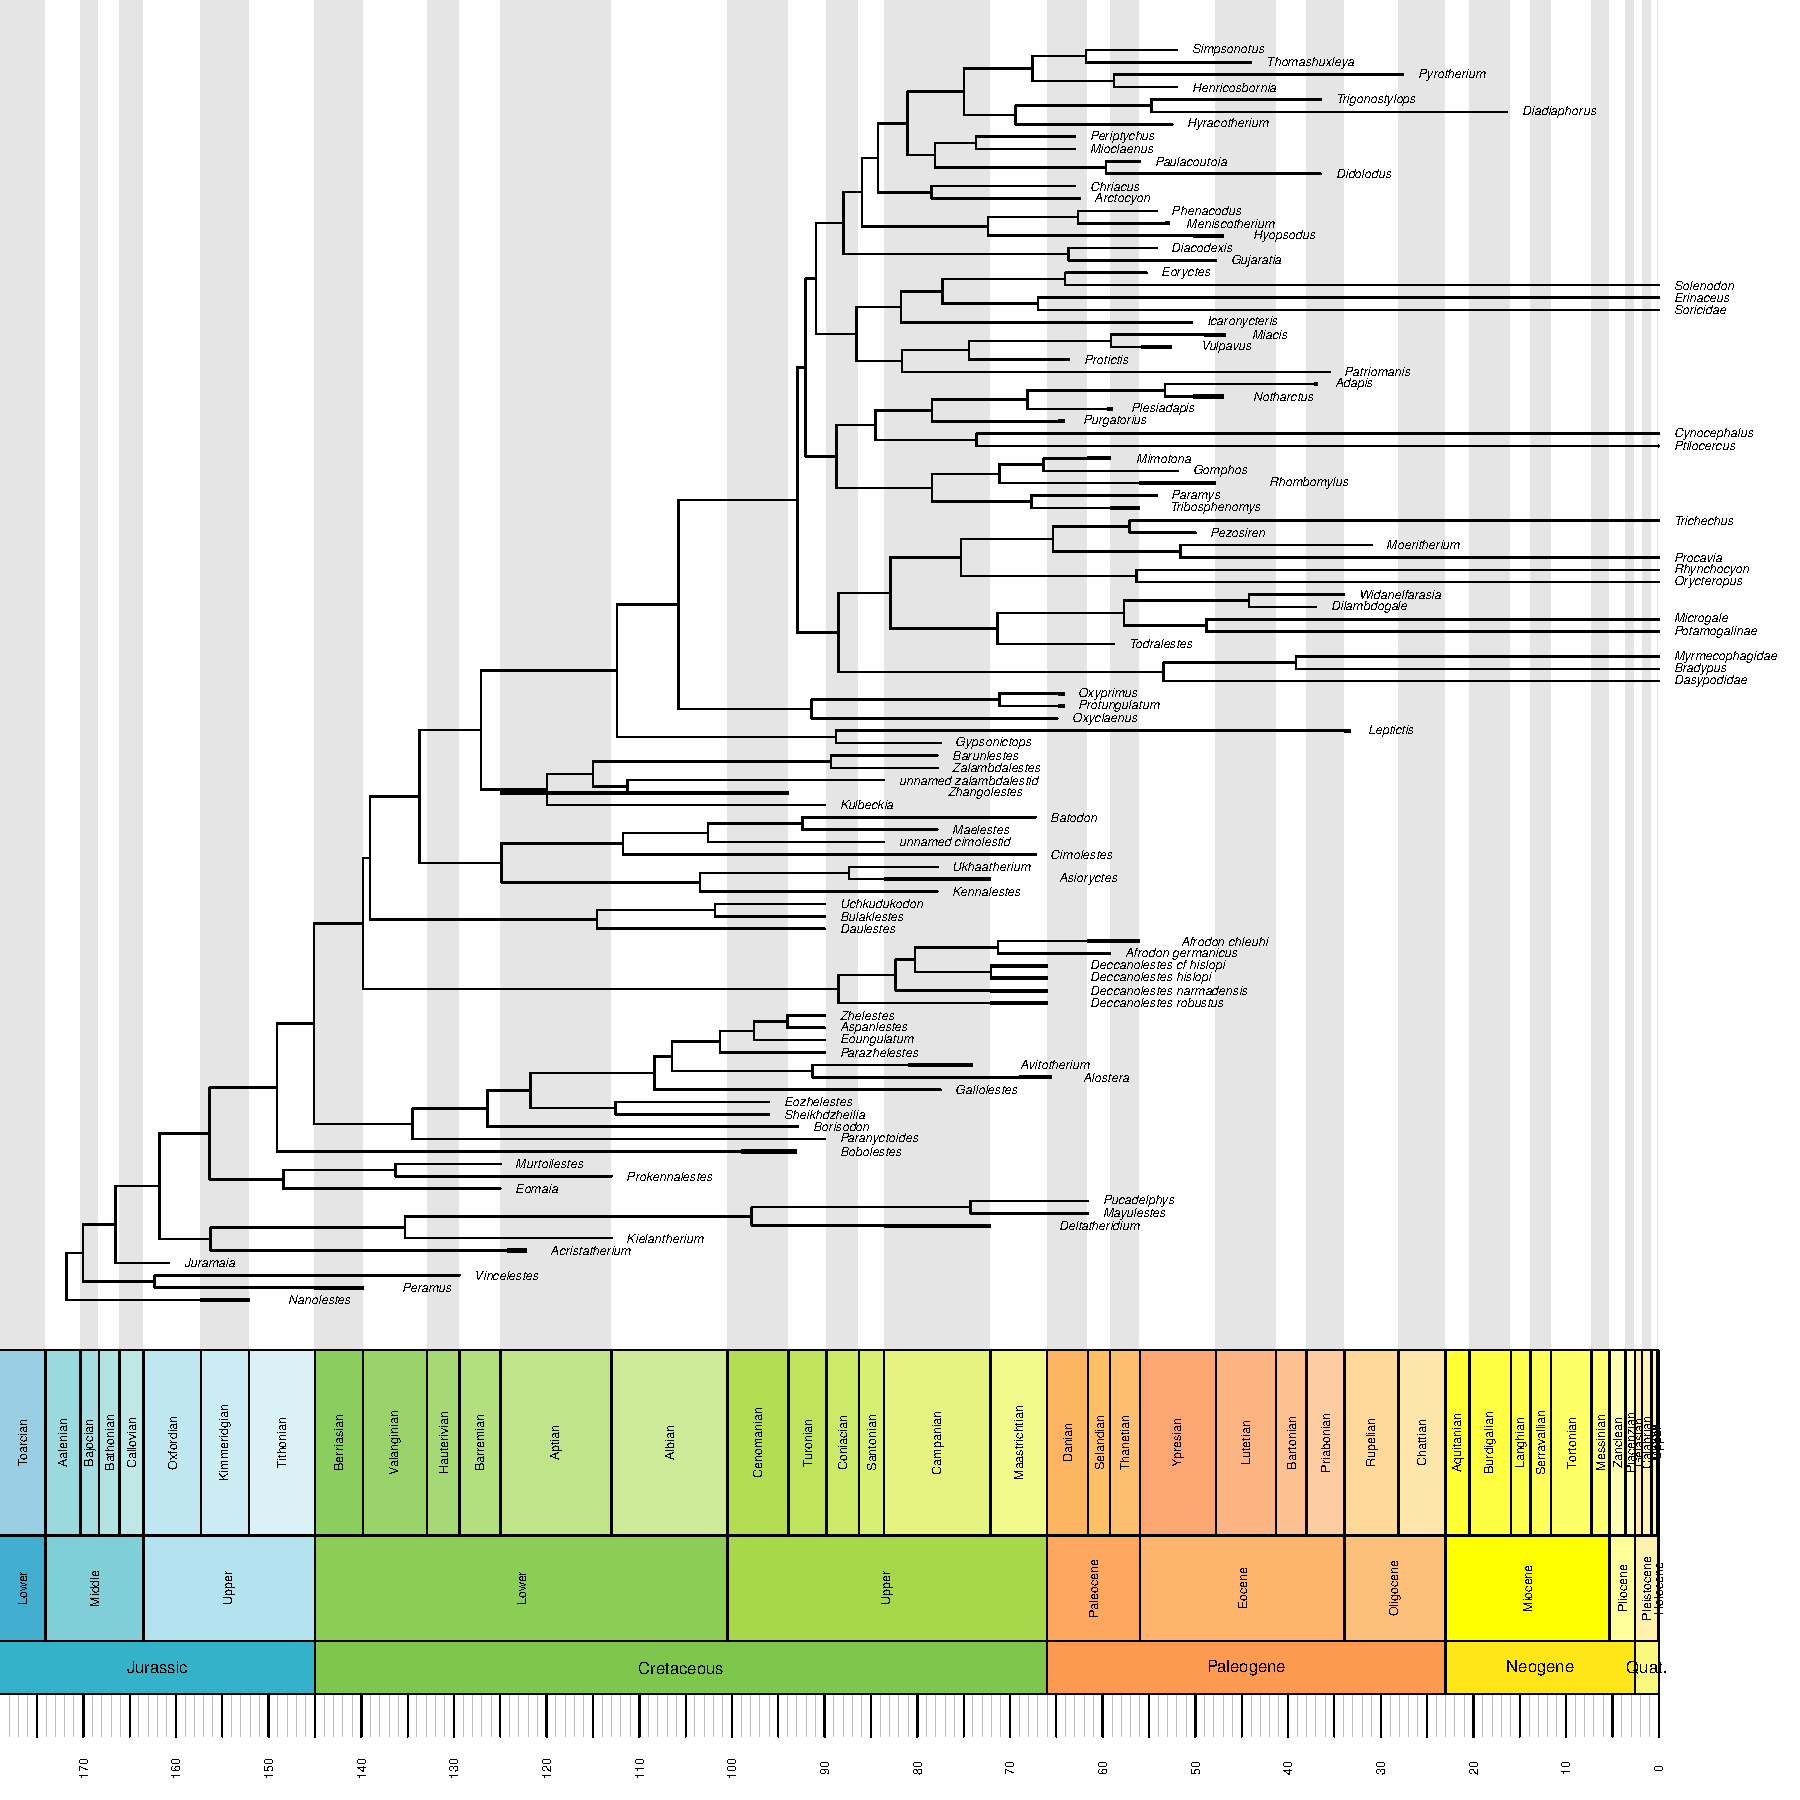
\includegraphics[width=1\linewidth, height=1\textheight, keepaspectratio]{figures/fig-tree-Beck2014-appendix.pdf}
    \caption[Beck2014.]
    {Phylogeny from Beck \& Lee (2014).}
    \label{figure:beck}
  \end{figure} 

\begin{figure}[!htbp]
    \centering
    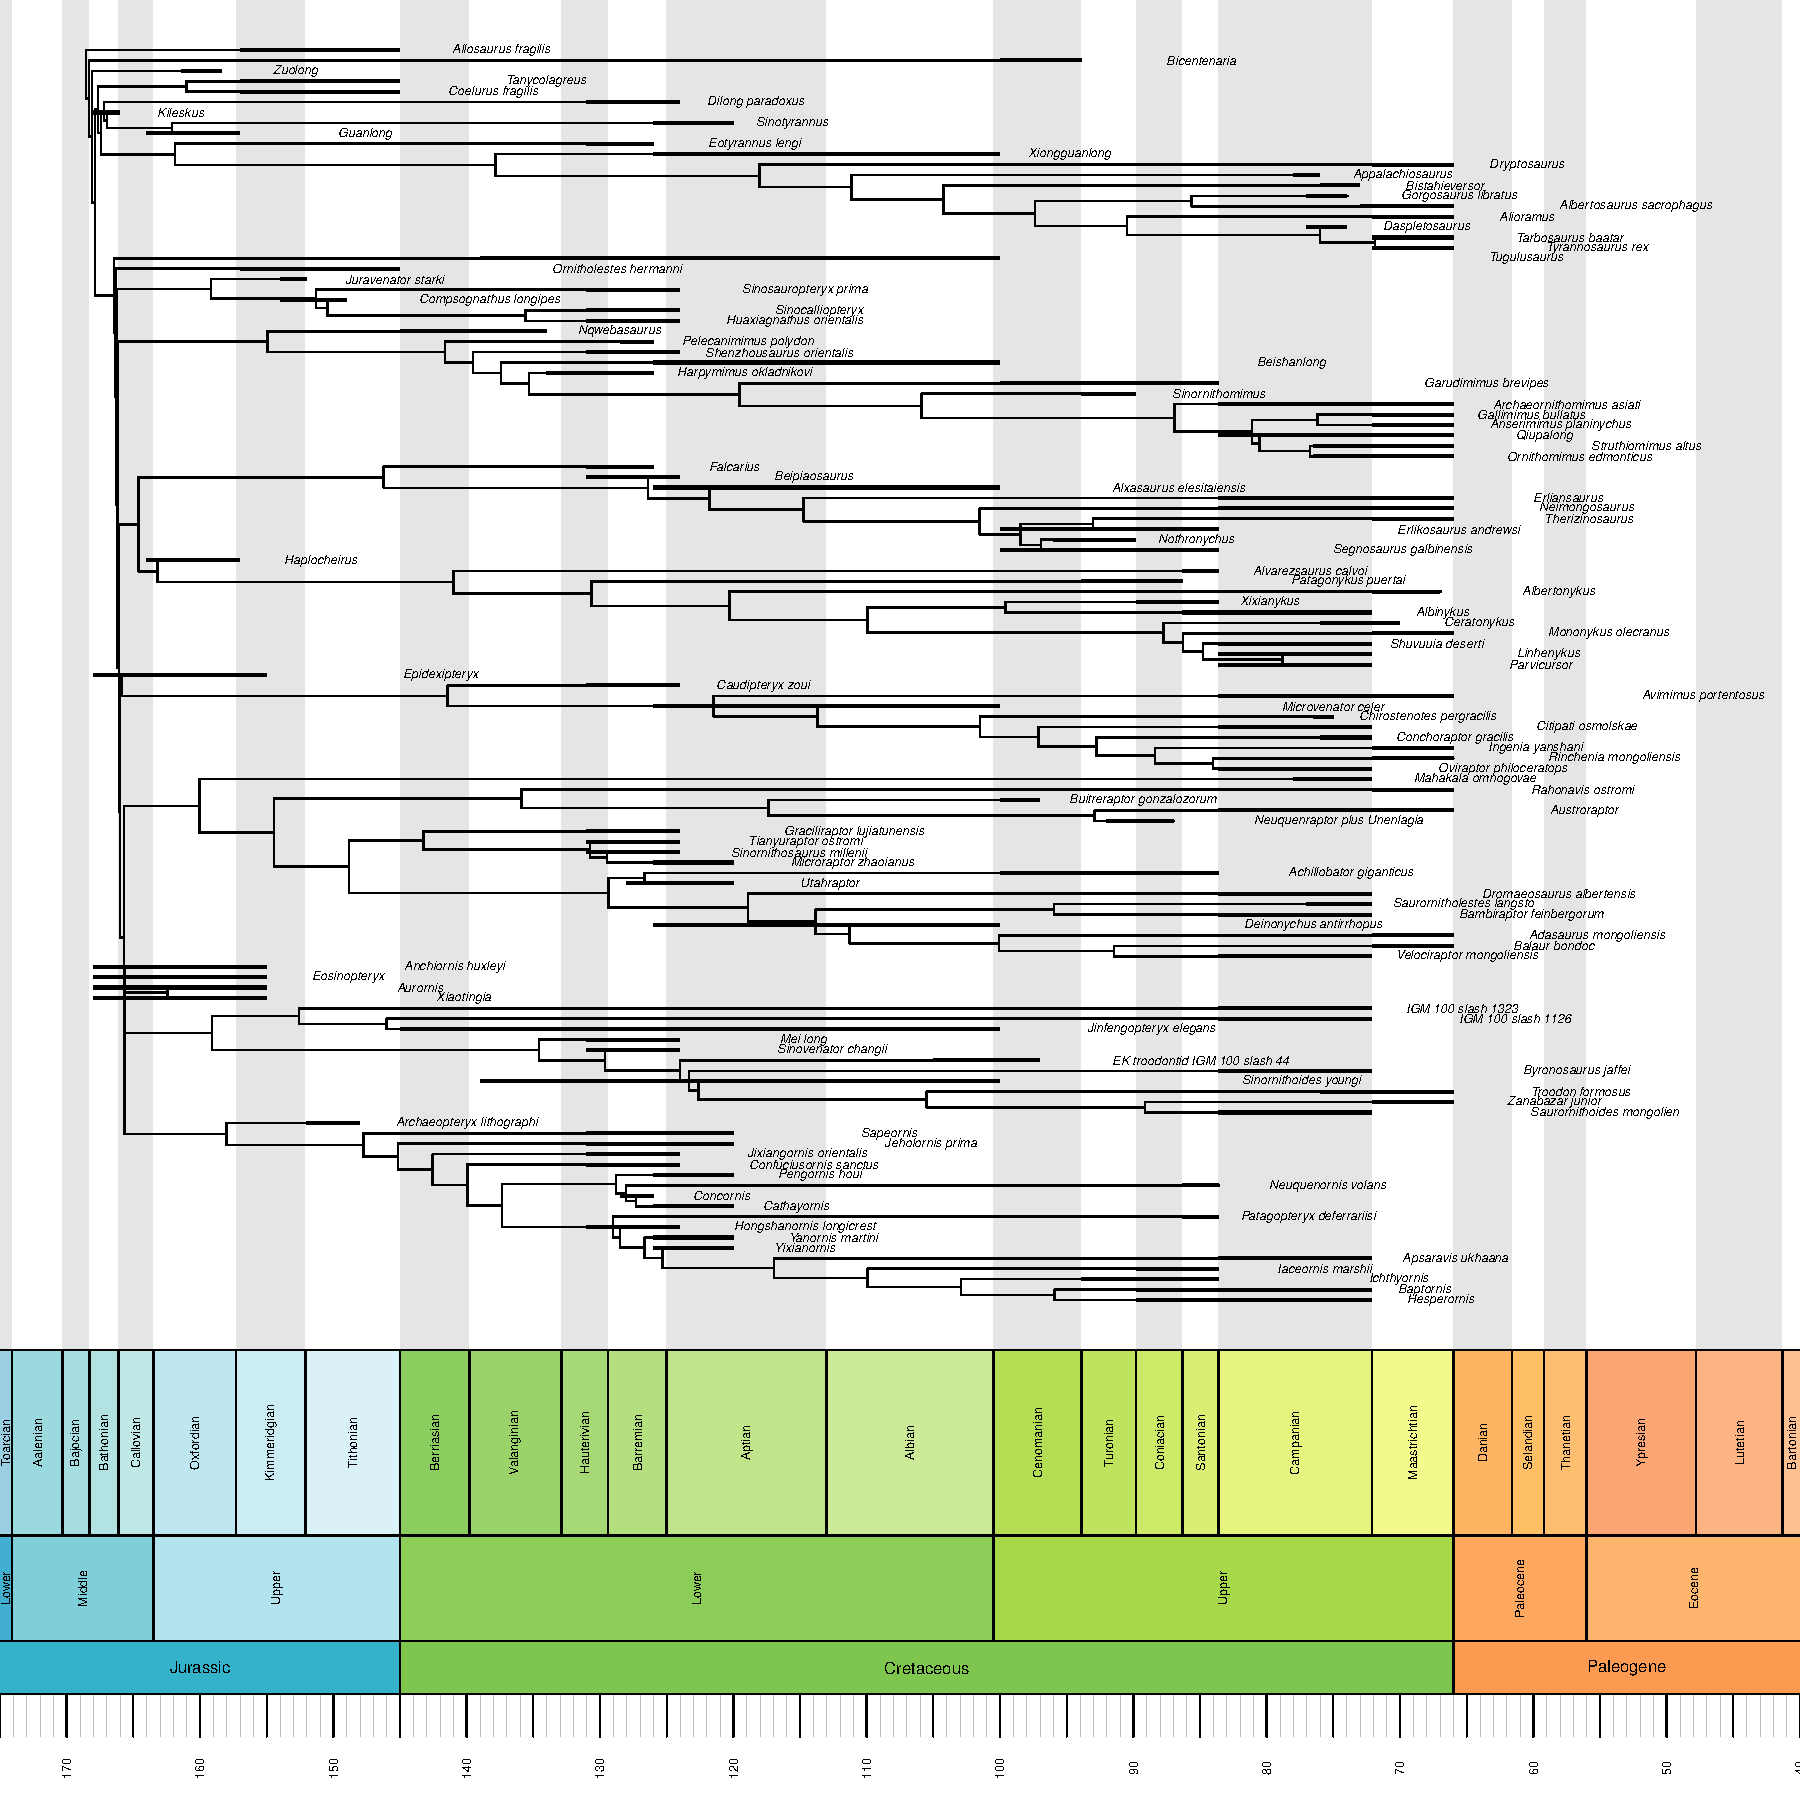
\includegraphics[width=1\linewidth, height=1\textheight, keepaspectratio]{figures/fig-tree-Brusatte2014-appendix.pdf}
    \caption[Brusatte2014.]
    {Phylogeny from Brusatte et al. (2014). This is one randomly selected tree from the time-scaled trees in the paper.}
    \label{figure:brusatte}
  \end{figure} 

\begin{figure}[!htbp]
    \centering
    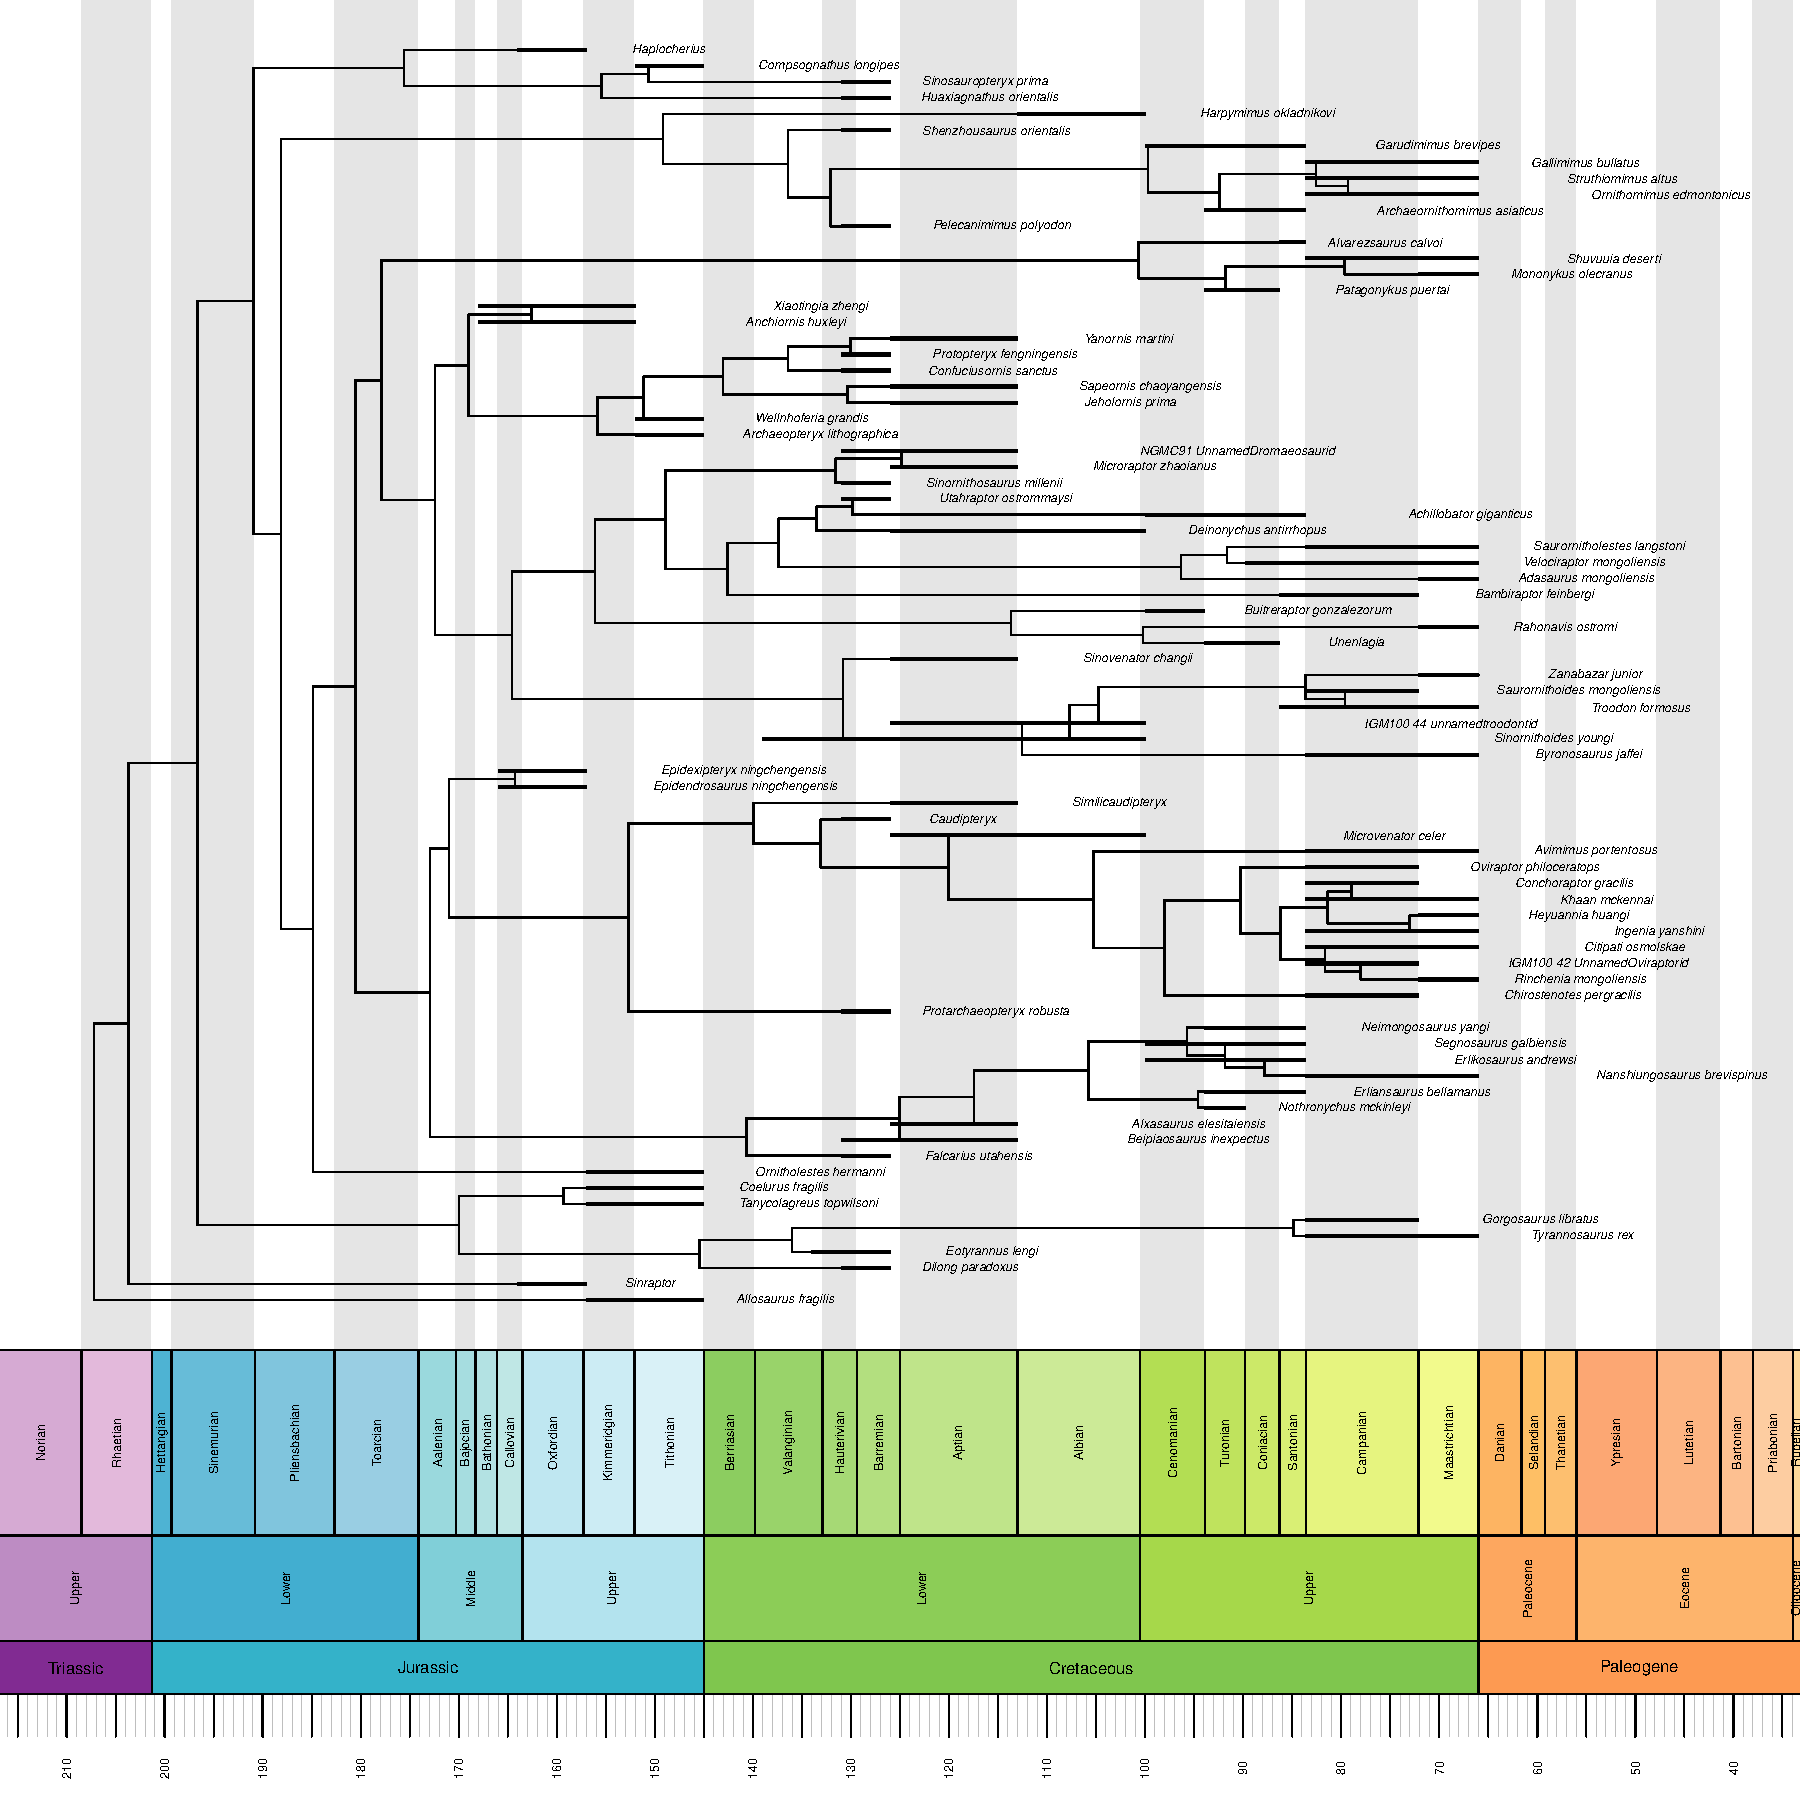
\includegraphics[width=1\linewidth, height=1\textheight, keepaspectratio]{figures/fig-tree-Bapst2016-appendix.pdf}
    \caption[Bapst2016.]
    {Phylogeny from Bapst et al. (2016). This is the maximum clade credibility tree.}
    \label{figure:bapst}
  \end{figure} 

\begin{figure}[!htbp]
    \centering
    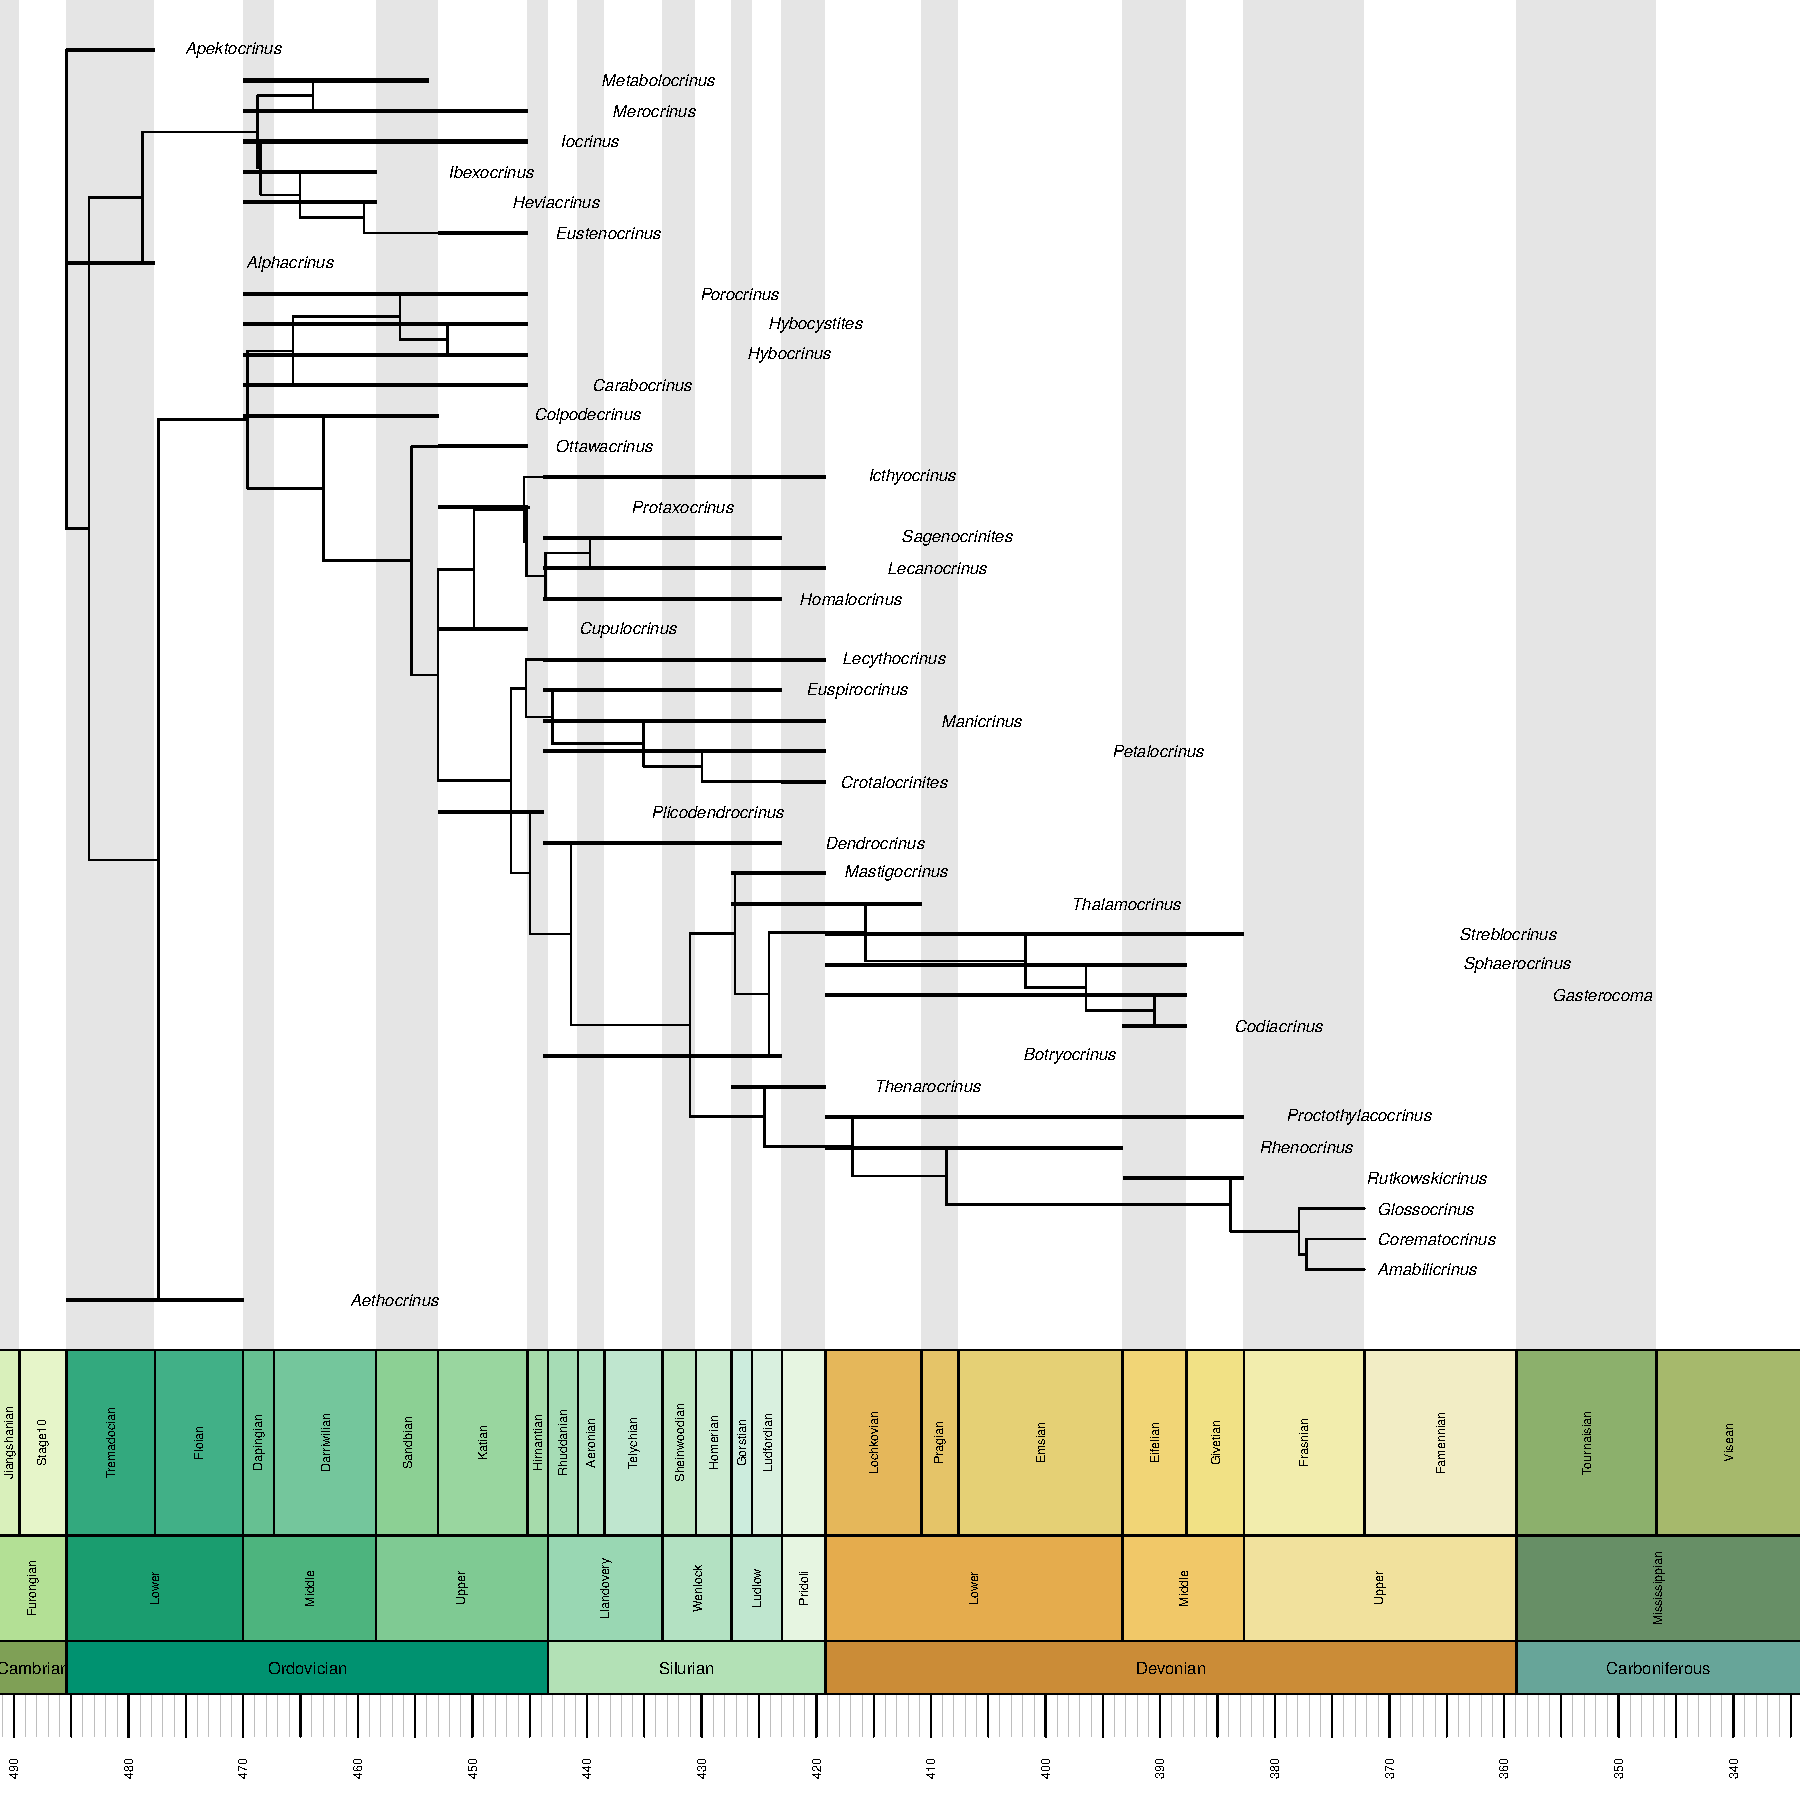
\includegraphics[width=1\linewidth, height=1\textheight, keepaspectratio]{figures/fig-tree-Wright2017-appendix.pdf}
    \caption[Wright2017.]
    {This is the maximum clade credibility tree from Wright (2017).}
    \label{figure:wright}
  \end{figure}  

\end{document}